\chapter{Fundamente}


\section{Rețea neurală}
O rețea neurală este un ansamblu interconectat de elemente de procesare simple, \textit{unități} sau \textit{noduri}, a căror funcționalitate este ușor bazată pe neuronul biologic. Abilitatea de procesare a rețelei este stocată în conexiunile inter-unități, sau \textit{ponderi} sinaptice, obținute dintr-un proces de adaptare la\ învățare dintr-un set de date de antrenare.\cite{Gurney:1997:INN:523781}

În biologie, fiecare neuron primește informație prin dendrite și transmite  informație prin axon, doar atunci când a primit suficientă informație de la neuronii conectați la dendritele sale. Astfel, un neuron va transmite informația mai departe atunci când cantitatea de informație primită depășește un anumit \textit{prag}.

Neuronii artificiali sunt construiți pe același principiu: dendritele vor fi echivalate de conexiuni către unitate, iar axonul de către o conexiune pornind de la acea unitate. Fiecare sinapsă( conexiune inter-neuronală) va fi caracterizată de o anumită \textit{pondere} astfel încât datele de intrare primite prin acea conexiune vor fi multipilicate cu acea pondere înainte de a fi transmise la neuronul artificial. Aici, semnalele ponderate sunt însumate pentru a forma o \textit{activare}.

În cadrul nodului, dacă \textit{activarea} va depăși un anumit \textit{prag}, unitatea va transmite mai departe o valoare(de obicei 1), altfel nu transmite nimic. Compararea cu pragul de activare se face folosind o funcție de activare. Procedeul descris (însumare, compararea cu pragul, apoi emiterea de 1 când pragul este mai mic și 0 altfel) reprezintă cel mai simplu model de neuron artificial, perceptronul.

\begin{figure}
    \begin{center}
        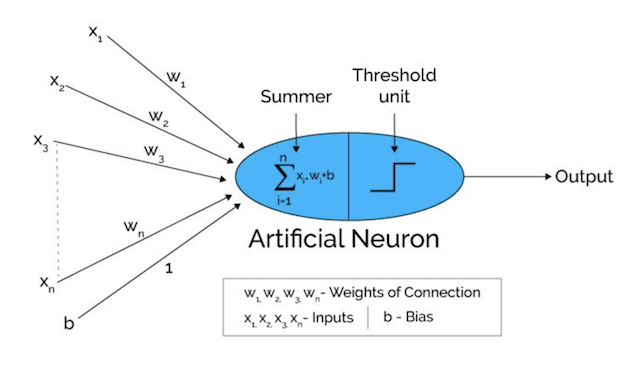
\includegraphics[width=0.7\textwidth]{images/perceptron.png}
         \caption{Un model de perceptron\cite{adi-from-perceptron}}
    \end{center}
\end{figure}
